\documentclass[12pt,aspectratio=169]{beamer}
\usetheme{default}
\usecolortheme{dolphin}
\usefonttheme{structurebold}
\setbeamertemplate{footline}[frame number]

\title{Network 05}
\author{@aoirint}
% \institute{}
\date{2020/06/25}

\begin{document}

% 01
\frame{\maketitle}

% 02
\begin{frame}{テキスト}

  \begin{minipage}{0.58\textwidth}
    \begin{itemize}
      \item ネットワークがよくわかる教科書
      \begin{itemize}
        \item 著・福永勇二
        \item 刊・SB Creative
      \end{itemize}
      \item 今回の内容
        \begin{itemize}
          \item Chapter 2、Section 12から13まで
        \end{itemize}

    \end{itemize}

  \end{minipage}
  \hfill
  \begin{minipage}{0.38\textwidth}
    \vspace{-1\baselineskip}
    \begin{figure}[h]
      \centering
      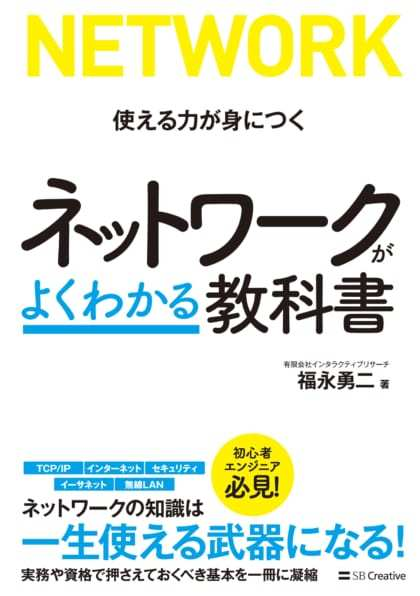
\includegraphics[width=4cm,bb=0 0 420 596]{../02/figures/networkbook.jpg}
      \label{fig:networkbook}
      \caption{テキスト}
    \end{figure}
  \end{minipage}

  \begin{itemize}
    \item 書影
    \begin{itemize}
      \item { \small \url{https://www.sbcr.jp/product/4797393804/} }
    \end{itemize}
  \end{itemize}

\end{frame}


\begin{frame}{今回の内容}

  \begin{itemize}
    \item ネットワークにおける通信
      \begin{itemize}
        \item ルーティングテーブルの役割
        \item IPパケットの分割と再構築
      \end{itemize}

  \end{itemize}

\end{frame}


\begin{frame}{ルーティングテーブル / Routing Table 1/2}

  \begin{itemize}
    \item 端末やルータが持つ、ある宛先IPのパケットを次にどのNICを介して、どこに送るべきか、という情報
    \item デフォルトルート / Default Route
      \begin{itemize}
        \item 適切な宛先が登録されていないときの設定(NIC、次の宛先)
      \end{itemize}
    \item デフォルトゲートウェイ(デフォルトルータ) / Default Gateway
      \begin{itemize}
        \item デフォルトルートとして設定されるルータ
        \item 複数のNICを持つ端末でも通常1つだけ指定
        \item 予備設定があることも % 使用中のデフォルトゲートウェイの故障時に切り替え
      \end{itemize}
    \item netstat -rn (Linux/Mac), netstat -r (Windows)

  \end{itemize}

\end{frame}


\begin{frame}{ルーティングテーブル / Routing Table 2/2}

  \begin{itemize}
    \item netstat -rn (Linux/Mac), netstat -r (Windows)
    \item ネットワークアドレス
    \item デフォルトルート
      \begin{itemize}
        \item 適切な宛先が登録されていないときの設定(NIC、次の宛先)
        \item 宛先:0.0.0.0
        \item ゲートウェイ:デフォルトゲートウェイのIPアドレス
      \end{itemize}
    \item ループバックインタフェース
      \begin{itemize}
        \item 127.0.0.1
        \item OSが用意する仮想的なNIC
        \item 自分自身あてのパケットが送られる
      \end{itemize}
    \item メトリック
      \begin{itemize}
        \item ルートの優先度(小さいほうが優先)
      \end{itemize}

  \end{itemize}

\end{frame}


\begin{frame}{IPパケットの分割と再構築 1/10}

  \begin{itemize}
    \item IPv4の機能(IPv6ではルータはフラグメンテーションしない) % ルータがこのような処理をするのは効率が悪い
    \item イーサネットの仕様上の制限
      \begin{itemize}
        \item 1フレームあたり1500バイトまで
      \end{itemize}

    \item ネットワークハードウェアの制限
      \begin{itemize}
        \item ハードウェアによって扱えるフレームの最大サイズが異なる % 規格・メモリの都合など?
      \end{itemize}

    \item ネットワークごとにパケットの最大サイズが異なる場合がある
      \begin{itemize}
        \item 異なるネットワーク間でパケットを中継するルータは、宛先ネットワークのパケット最大サイズを考慮する必要がある
      \end{itemize}

    \item IPフラグメンテーション
      \begin{itemize}
        \item ルータによるIPパケットの分割
      \end{itemize}

  \end{itemize}

\end{frame}


\begin{frame}{IPパケットの分割と再構築 2/10}

  \begin{enumerate}
    \item 送信元コンピュータからパケットが送出される
    \item 中継するルータがパケットを分割する
      \begin{itemize}
        \item 経路には複数のルータが考えられる
      \end{itemize}
    \item 受信側コンピュータが分割されたパケットを復元する

  \end{enumerate}

\end{frame}


\begin{frame}{IPパケットの分割と再構築 3/10}

  \begin{itemize}
    \item MTU / Maximux Transmission Unit
      \begin{itemize}
        \item ネットワークハードウェアが一度に送信できる最大データサイズ
        \item IPでは576バイト以上でなければならない
      \end{itemize}
    \item MTUの小さなネットワーク(ルータ)にパケットを送信するとき、分割する必要がある
      \begin{itemize}
        \item コンピュータの内部では事前にMTUを考慮するのでふつうIPフラグメンテーションは発生しない
        \item ルータがパケットを中継するとき分割が起こる
      \end{itemize}

  \end{itemize}

\end{frame}


\begin{frame}{IPパケットのフォーマット(前回のスライド)}

  \centering
  \begin{figure}
    \centering
    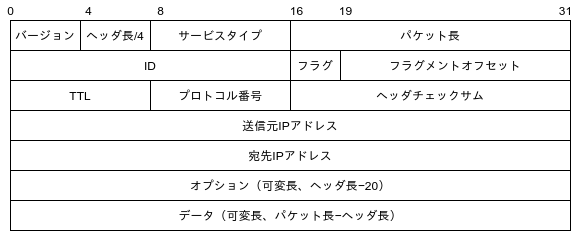
\includegraphics[width=12cm,bb=0 0 581 232]{../04/figures/ip_packet.png}
    \label{fig:ip_packet}
    \caption{IPパケットのフォーマット(IPv4)}
  \end{figure}

\end{frame}


\begin{frame}{IPパケットの分割と再構築 4/10}

  \begin{itemize}
    \item 使用するフィールド
      \begin{itemize}
        \item ID、フラグ、フラグメントオフセット
        \item データ(分割したデータを格納)
      \end{itemize}
    \item 影響を受けるフィールド
      \begin{itemize}
        \item パケット長、ヘッダチェックサム
      \end{itemize}
    \item 同時に書き換えられるフィールド
      \begin{itemize}
        \item TTL
      \end{itemize}

    \item 他の層のことは考慮しなくてよい
      \begin{itemize}
        \item 受信者はパケットを再構築(分割されたデータを結合)してから使用する
        \item イーサネットフレームはIPフラグメンテーションの適用有無にかかわらず中継のたびに作られる
      \end{itemize}

  \end{itemize}

\end{frame}


\begin{frame}{IPパケットの分割と再構築 5/10}

  \begin{itemize}
    \item パケットの分割
    \item ID
      \begin{itemize}
        \item もとのパケットと同じ値を設定する
      \end{itemize}
    \item フラグ
      \begin{itemize}
        \item 「後続フラグメントあり」を使用する
        \item 分割されたパケットの末尾なら0、それ以外なら1を設定
      \end{itemize}
    \item フラグメントオフセット
      \begin{itemize}
        \item この分割がもとのデータの先頭何バイト目から始まっているか
        \item その値を8で割った値を格納
      \end{itemize}

  \end{itemize}

\end{frame}

\begin{frame}{IPパケットの分割と再構築 6/10}

  \begin{figure}
    \centering
    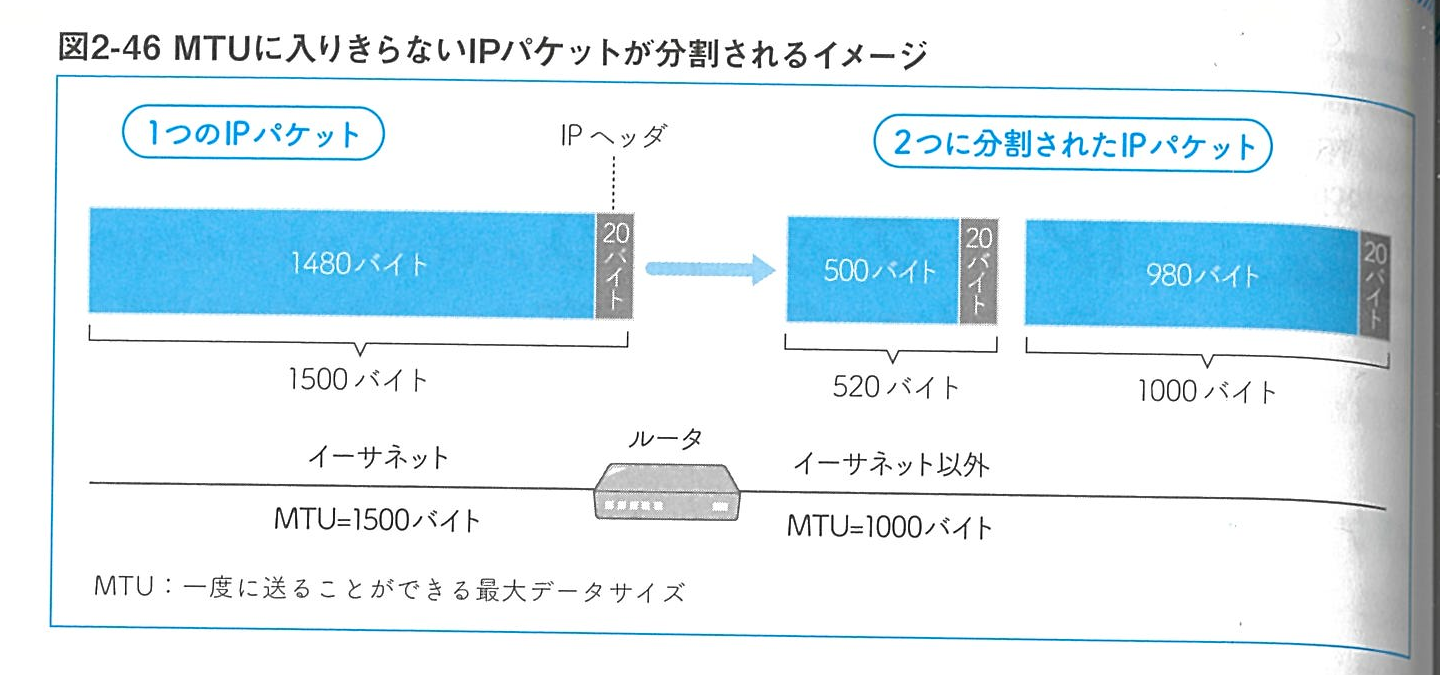
\includegraphics[width=10cm,bb=0 0 1440 675]{figures/ip_fragm1.png}
    \label{fig:ip_fragm1}
    \caption{IPパケットの分割(IPv4)、テキストp82から引用}
  \end{figure}

\end{frame}

\begin{frame}{IPパケットの分割と再構築 7/10}

  \begin{figure}
    \centering
    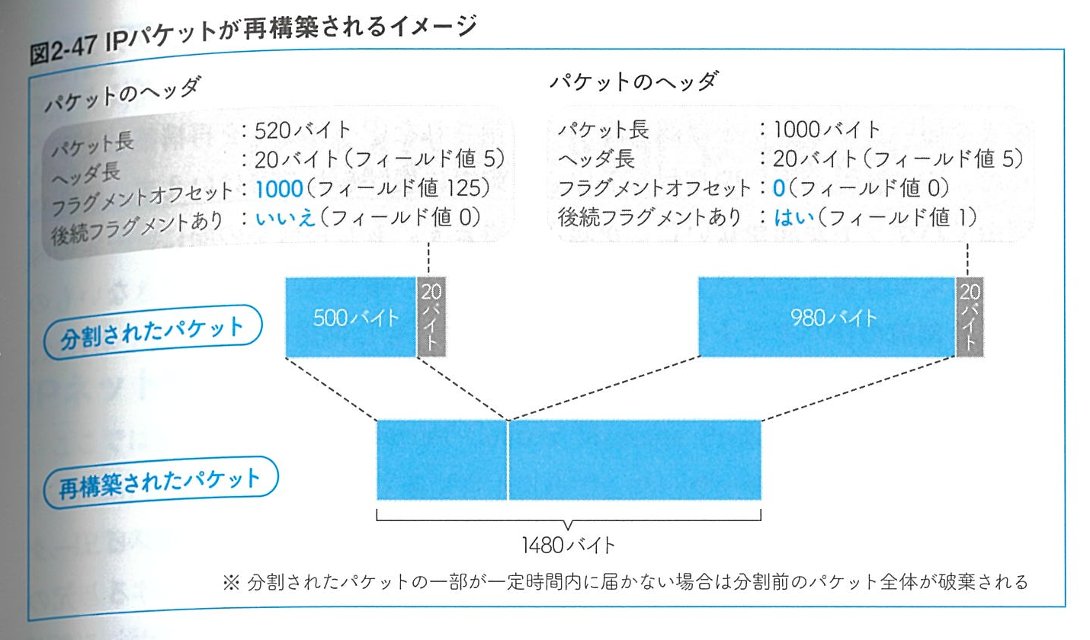
\includegraphics[width=10cm,bb=0 0 1090 640]{figures/ip_fragm2.png}
    \label{fig:ip_fragm2}
    \caption{IPパケットの再構築(IPv4)、テキストp83から引用}
  \end{figure}

\end{frame}

\begin{frame}{IPパケットの分割と再構築 8/10}
  \begin{itemize}
    \item パケットの再構築
      \begin{itemize}
        \item 受信側のコンピュータで行う(ルータではない)
      \end{itemize}
    \item バラバラの順で届くフラグメントを結合する
      \begin{itemize}
        \item フラグメントオフセットでデータの先頭位置がわかる
        \item 「後続フラグメントあり」フラグでデータの末尾がわかる
      \end{itemize}
    \item フラグメントの一部が届かなかったとき
      \begin{itemize}
        \item そのパケットの受信したフラグメントすべてを破棄する
      \end{itemize}

  \end{itemize}

\end{frame}


\begin{frame}{IPパケットの分割と再構築 9/10}
  \begin{itemize}
    \item 分割禁止フラグ
      \begin{itemize}
        \item IPパケットのフラグの1つ
        \item 1のとき、IPフラグメンテーションしない
        \item 分割が必要になったとき、そのパケットを破棄する
        \item パケットが破棄されたことはICMPによって通知される
      \end{itemize}

  \end{itemize}

\end{frame}


\begin{frame}{IPパケットの分割と再構築 10/10}

  \begin{itemize}
    \item Path MTU Discovery
      \begin{itemize}
        \item 効率の悪い「ルータでのパケットの分割」という操作を極力避けるための手法の1つ
        \item TCP、UDPがサポート
        \item ICMPを使って経路上で分割が発生しないMTUサイズを検出する
        \item あらかじめコンピュータ上でパケットサイズを適切なMTUに合わせる
      \end{itemize}
    \item Path MTU Discoveryブラックホール
      \begin{itemize}
        \item ICMPパケットを遮断する機器が経路に含まれているときうまく機能しないことがある
      \end{itemize}
  \end{itemize}

\end{frame}

\end{document}
